\chapter{Strategy}
\label{sec:strategy}

In this chapter, we present our strategy that helps with the identification of rules to avoid the generation of useless mutants. 
We explain the strategy in Section~\ref{sec:strategy-identifying}. 
Then, we evaluate the strategy in Section~\ref{sec:strategy-evaluation}.
Finally, we discuss the research status in Section~\ref{sec:research-status-strategy}


\section{Identifying Useless Mutants Candidates}

\label{sec:strategy-identifying}

Our strategy is based on three inputs. 
The first one comprises a set of programs. 
For each program, the strategy also needs a green test suite and a set of mutants. 
Figure~\ref{fig:strategy} illustrates the strategy. 
First, we collect the set of programs (Step~1). 
Steps~2 and~3 collect a passing test suite and a set of mutants for each program of the Step~1. 
For each mutant gathered in Step~3, we execute all tests of Step~2 and collect the results (Step~4). 
In the last step, we identify potential candidates of equivalent and duplicated mutants (Step~5).

To classify the mutants as equivalents or duplicated candidates, the strategy proceeds as follows. 
Given a program \textit{P}, when its test suite \textit{T} is executed in a mutant \textit{M} (generated from \textit{P}) and \textit{T} does not have any failing test case, \textit{M} seems to not change the behavior of the original program \textit{P}. 
This way, the strategy sets \textit{M} as an equivalent mutant candidate. 
If two mutants generated from \textit{P} (\textit{M$_i$} and \textit{M$_j$}) have the same non-empty set of failing test cases in \textit{T}, the strategy sets \textit{M$_i$} and \textit{M$_j$} as duplicated mutants.

We are classifying mutants as useless or useful according to \textit{strong kill}, that is, for a given program \textit{P}, a mutant \textit{M} of program \textit{P} is said to be killed only if mutant \textit{M} gives a different output from the original program \textit{P}.

Notice that our strategy is flexible in the sense we can collect programs, test suites, and mutants from different tools and setups. 
In Figure~\ref{fig:strategy}, we illustrate the strategy using a program generator named \jdolly{}~\cite{SOARES:2013:1}, a test suite generator (\randoop{}~\cite{PACHECO:2007:1}), and a mutation testing tool to generate mutants of a given program, e.g., \pit{}~\cite{PIT:2017}.

\begin{figure*}[ht]
	\begin{center}
		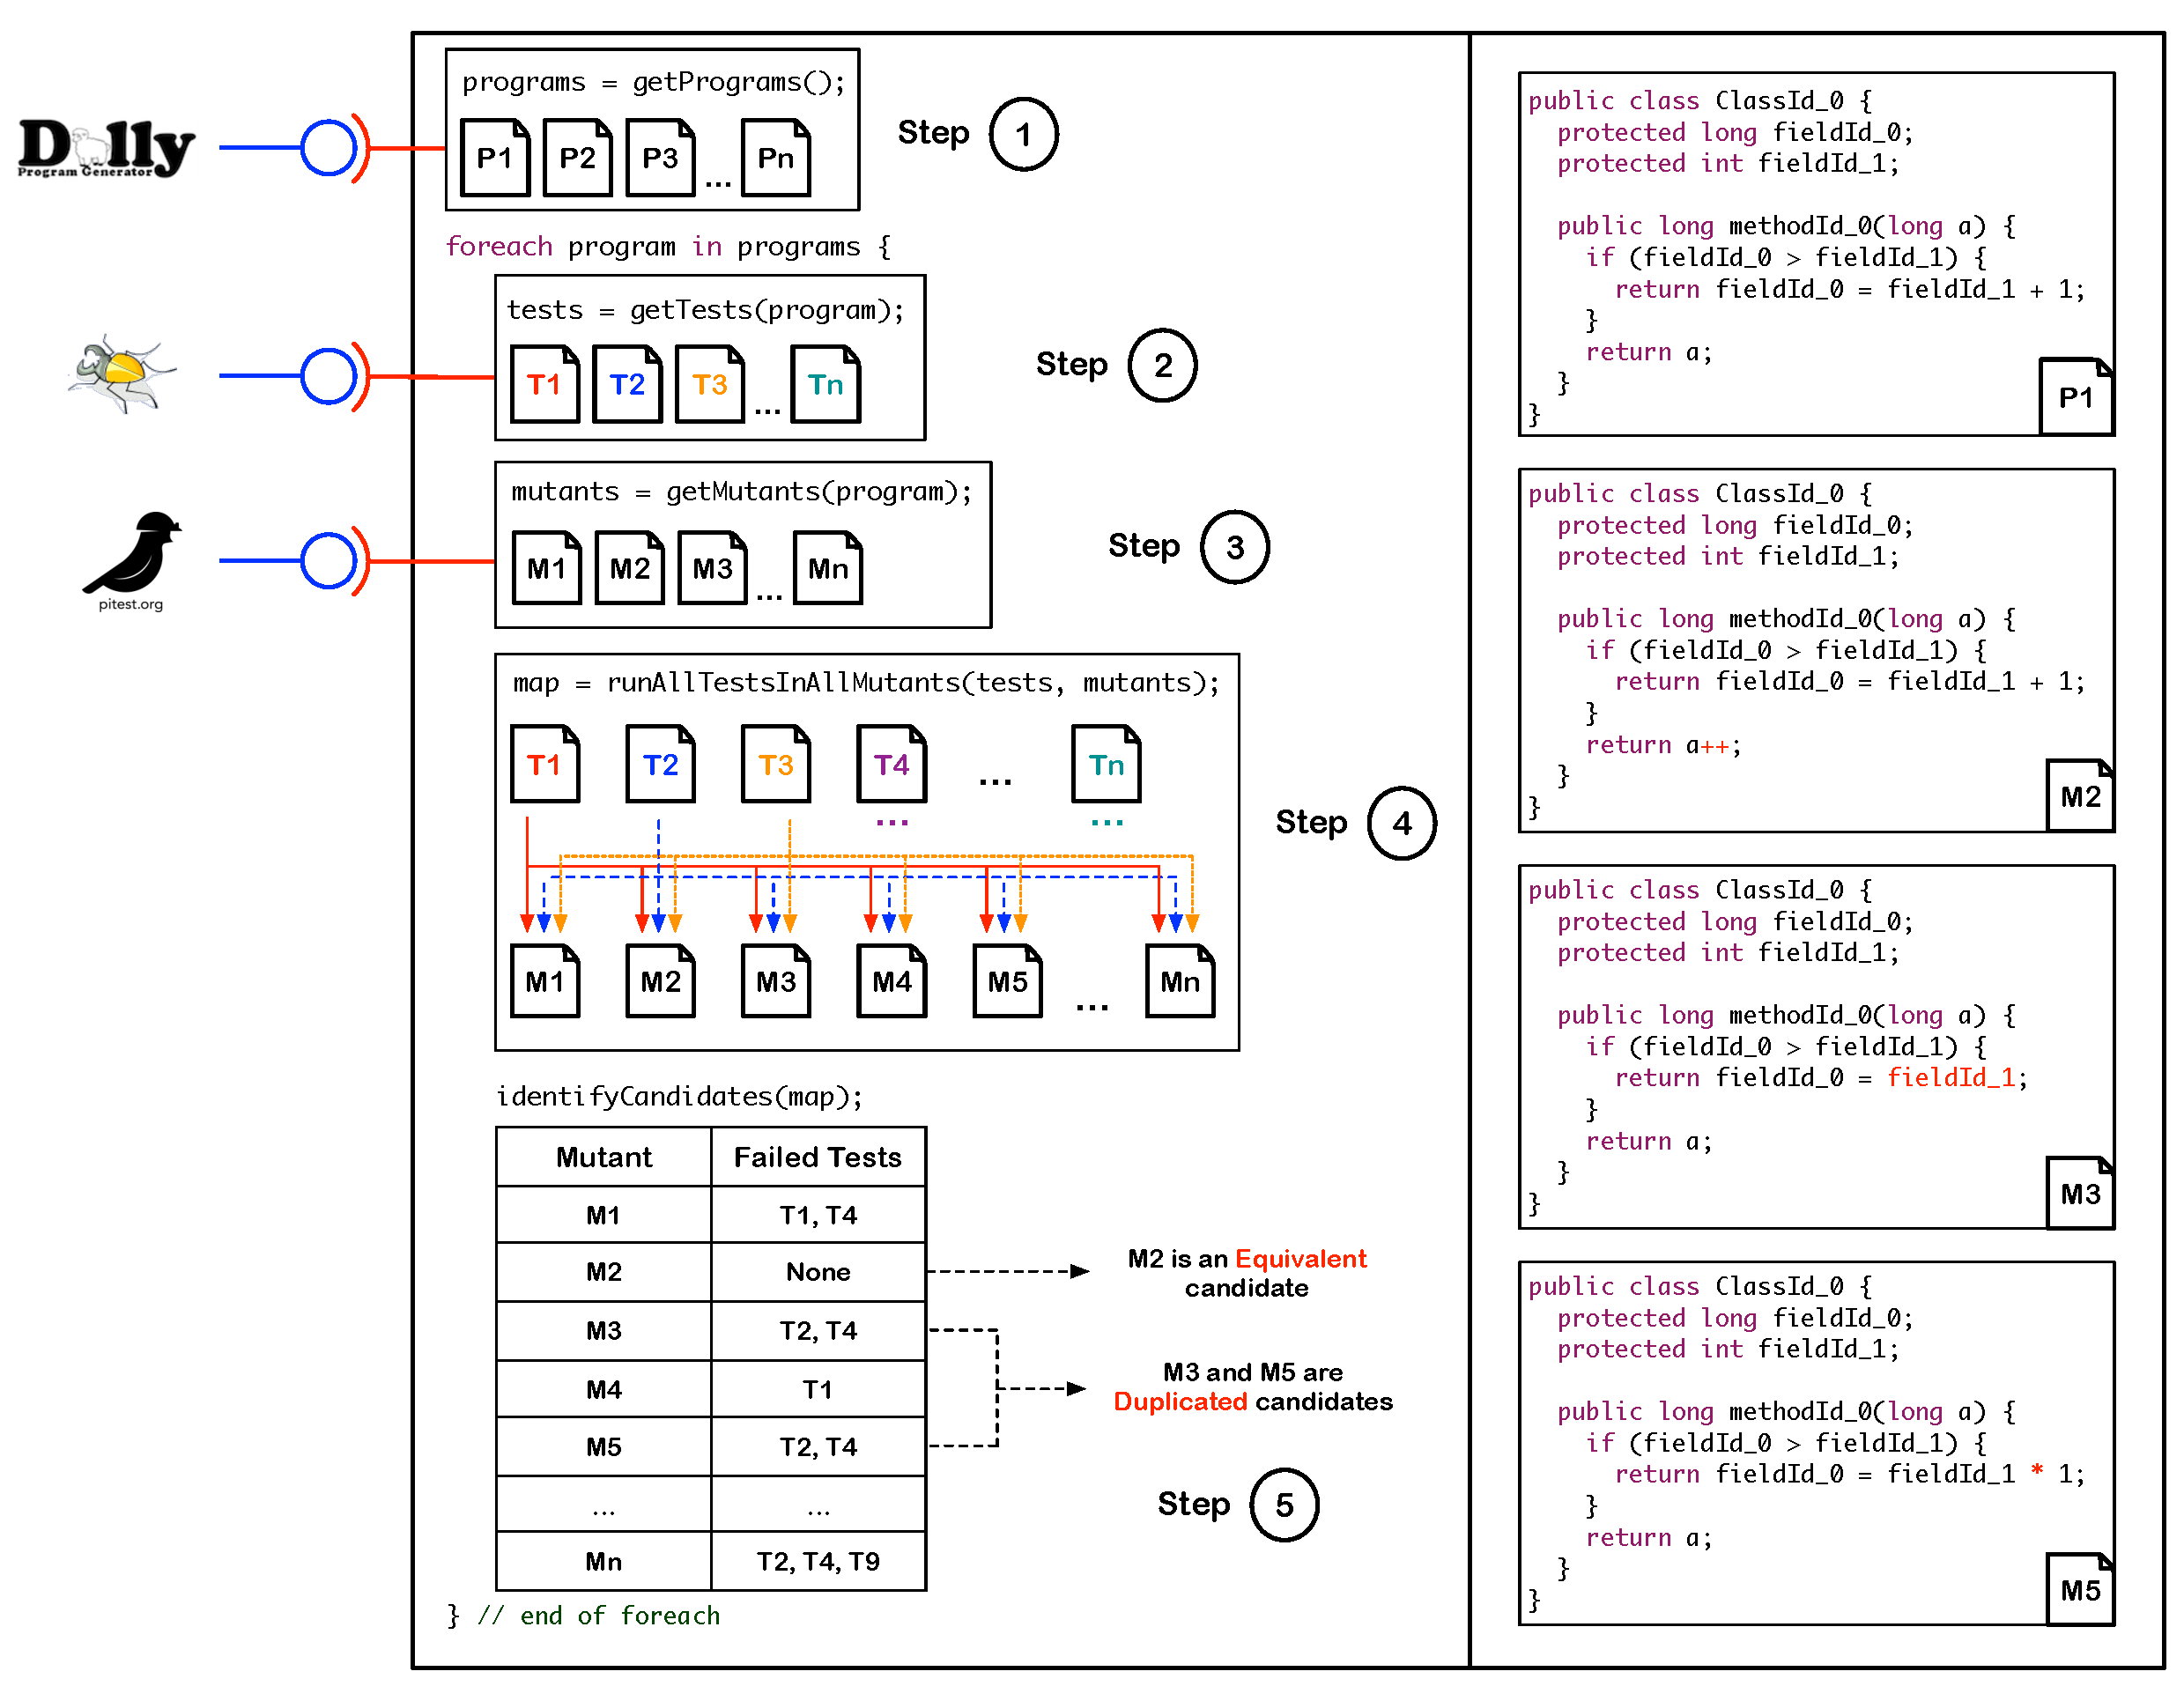
\includegraphics[scale=0.35]{images/Strategy.pdf}
		\caption{Strategy to identify equivalent and duplicated mutants candidates.}
		\label{fig:strategy}
	\end{center}
\end{figure*}


\section{Evaluation}
\label{sec:strategy-evaluation}

In this section, we execute our strategy to identify useless mutants candidates. 
By analyzing these candidates, we derive rules to avoid their generation (see Chapter~\ref{sec:rules}). 
We present the settings of our execution and then we discuss the results.

\subsection{Settings}

We intend to answer the following research question: \textit{Is the strategy capable of identifying useless mutants candidates?} 
To answer this question, we instantiate our strategy with \jdolly{}~\cite{SOARES:2013:1} to generate the set of programs; \randoop{} \cite{PACHECO:2007:1} as our test suite generator; and \mujava{}~\cite{OFFUTT:2005:1, OFFUT:2006:1}, \major{}~\cite{JUST:2011:1}, and \pit{}~\cite{PIT:2017} as our mutants generators.

\jdolly{} is an automated and bounded-exhaustive Java program generator based on Alloy, a formal specification language~\cite{alloy-book}. 
\jdolly{} receives as input an Alloy meta-model, which comprises a subset of possible Java constructs, and a scope, which is the maximum number of elements (classes, methods, fields, and packages) that the generated programs may declare, and optional constraints for guiding the program generation. 
It uses the Alloy Analyzer tool~\cite{alcoa}, which takes an Alloy specification and finds a finite set of all possible instances that satisfy the constraints within the specified scope. 
\jdolly{} then translates each instance found by the Alloy Analyzer to a Java program. 
It reuses the syntax tree available in Eclipse JDT for generating programs from those instances. 
Program \textit{P1} in Figure~\ref{fig:background} is a program generated by \jdolly{}. 

We execute our strategy to analyze \AnalyzedPrograms programs generated using \jdolly{}. 
In particular, we set \jdolly{} to generate programs with at most three fields (with or without overwriting), three methods (with or without overwriting and overloading), and two classes. 
One class always extends the other one. 
We also set \jdolly{} to use only the \texttt{int} and \texttt{long} primitive types. 
A class is the only non-primitive type. 
Moreover, each class is located into a package. 
If a class is not explicitly related to a package, the default package is assumed. 
Each field is associated with one identifier, one type, and at most one modifier, which can be protected or private. 
A method declaration contains a return type, an identifier, a parameter, a body, and a modifier related to its accessibility, which can be protected or public.

Since we use small and artificially-generated programs with no test suite, we  use \randoop{} as our test suite generator.
\randoop{}\footnote{\randoop{} stands for ``random tester for object-oriented programs''.}~\cite{PACHECO:2007:1} is an automatic unit test generator for Java. 
It generates unit tests, in JUnit format, using feedback-directed random test generation.
This means that it uses feedback obtained from executing a sequence of method calls and constructor invocation to create and mutate objects as it is being constructed. Then, it  uses this sequence of method calls plus an assertion about the result of a final method call to create the test.
Two types of tests are generated: error-revealing tests and regression tests. 
Error-revealing are tests that fail when executed, indicating a potential error in one or more classes under test.
Regression tests are tests that pass when executed and are useful in the future after a change in code.
%If the test passes right after its generation and it failures after a code change, then the change may have altered the program behavior.
\randoop{} is fully automatic, requires no input from the user (other than a class directory for Java) and, optionally, a time limit to generate tests. 
Previous experiments \cite{PACHECO:2007:1, PACHECO:2008:1} have shown that \randoop{} scales to realistic applications with hundreds of classes, which allowed it to find bugs in widely-deployed commercial and open-source software.

We acknowledge that the programs generated with \jdolly{} have a reduced scope when compared to industrial-scale systems and that random tests do not perform well for complex systems~\cite{ARTHO:2016:1} when compared with manually-made tests.
Nevertheless, previous work was capable of finding bugs in refactoring engines (e.g., Eclipse, JRRT, and NetBeans) by using a similar scope in \jdolly{} and with tests generated by \randoop{}~\cite{SOARES:2010:1, SOARES:2013:1, MONGIOVI:2014:1, MELINA:2017:1}.

%Given that our programs and the test set were built around the Java language, we search for Java mutation testing tools to generate the mutants.
%In the context of Software Engineering conferences, the three widely-used mutation testing tools for Java are \mujava{}, \pit{}, and \major{} \cite{KINTIS:2016:1}.
%So we chose those tools for our evaluation.

Regarding mutation testing tools, we selected \mujava{}, \pit{}, and \major{}.
These tools have different mutation operators.
In this evaluation, we use all available mutation operators of each tool (47 from \mujava{}, 9 from \major{}, and 13 from \pit{}).

%The next step of our strategy is to get all tests generated from each program and run against their respective mutants (Step~4). 
%The output of this is a table similar to that found in Figure \ref{fig:strategy} for each program.
%With this information, the strategy classifies the mutants as useful or useless (equivalent or duplicated) (Step~5).

%To check whether the mutants classified as useless are indeed useless, we manually analyze all of them together with the \AnalyzedPrograms programs.
It is important to note that we chose to use simple programs generated by \jdolly{}, instead of using complex Java programs, because it makes our entire evaluation feasible, since we wanted to explore all mutation operators from all mutation tools.
In addition, simple programs facilitate the manual analyses and minimize noise when reading and understanding the original and mutated programs.

\subsection{Results and Discussion}

We now present the results to answer our research question. 
As mentioned, we generated \AnalyzedPrograms programs based on \jdolly{}. 
The mutants generators yielded 4,999 mutants. 
Our strategy classified 963 mutants as equivalents and 1,332 mutants as duplicated. 
Table~\ref{tab:number-mutants} presents the results. 
Although we are using artificially generated programs, the numbers of equivalents and duplicated mutants are similar to the numbers presented in recent works~\cite{KINTIS:2017:1, KINTIS:2016:1}.

\scriptsize
\begin{table}[ht]
	\centering
	\caption{Useless mutants candidates identified.}
	\label{tab:number-mutants}
	\begin{tabular}{|l|c|c|c|}
		\hline
		& \textbf{Mutants} & \textbf{Equivalents}  & \textbf{Duplicated}    \\ \hline
		\mujava{} & 3,170    & 592 (18.6\%) & 1,089 (34.3\%) \\ \hline
		\major{}  & 816     & 166 (20.3\%) & 83 (10.1\%)   \\ \hline
		\pit{}    & 1,013    & 205 (20.2\%) & 160 (15.7\%)  \\ \hline
		TOTAL  & 4,999    & 963 (19.2\%) & 1,332 (26.6\%)  \\ \hline
	\end{tabular}
\end{table}
\normalsize

We detected some false positives, i.e., the strategy classified mutants as useless, but they are not. 
Table~\ref{tab:confusion-table} presents a confusion matrix to summarize our results. 
From 4,999 generated mutants (n), our strategy pointed 2,295 as useless and 2,704 as useful. 
Our manual analysis classified 204 out of 2,295 as false positives (FP) and 2,091 as true positives (TP). 
Notice that we did not have false negatives (FN) since our strategy found tests capable of killing all mutants pointed as useful. 
These numbers give us an accuracy of 95.92\%. 
When analyzing the false positives, we observed that some branches have not been covered by the test suite. 
It occurred because \randoop{} does not use techniques like symbolic execution~\cite{CORINA:2010:1}. 
This way, the generated tests could not kill any of the mutants that mutated code within such branches. 
This means that the quality of the test cases and their coverage play an important role in reducing false positives.

\scriptsize
\begin{table}[ht]
	\centering
	\caption{Confusion Matrix.}
	\label{tab:confusion-table}
	\begin{tabular}{|c|c|c|r|}
		\hline
		\multicolumn{2}{|c|}{\multirow{2}{*}{\textbf{n = 4,999}}} & \multicolumn{2}{c|}{\textbf{Actual}}                                 \\ \cline{3-4} 
		\multicolumn{2}{|c|}{}                                   & \textbf{true}                  & \multicolumn{1}{c|}{\textbf{false}} \\ \hline
		\multirow{2}{*}{\textbf{Predicted}}   & \textbf{true}    & \multicolumn{1}{r|}{2,091 (TP)} & 204 (FP)                            \\ \cline{2-4} 
		& \textbf{false}   & \multicolumn{1}{r|}{0 (FN)}    & 2,704 (TN)                           \\ \hline
	\end{tabular}
\end{table}
\normalsize

% We analyze the mutation operators more prone to generate useless mutants.
% Figure~\ref{fig:operators-equivalent} illustrates the number of equivalent mutants based on some mutation operators. 
% The AOIS operator (showed in Figure~\ref{fig:background}) was the one that generated the highest number of equivalent mutants. 
% This happens due to the several \texttt{return} statements generated by \jdolly{}. 
% Figure~\ref{fig:operators-duplicated} illustrates the number of duplicated mutants based on some mutation operators. 
% An example of two operators that together generated many useless mutants is COI (Conditional Operator Insertion) and ROR (Relational Operator Replacement).
% Given the following conditional expression \texttt{(x < y)}, COI generated \texttt{!(x < y)} whereas ROR generated \texttt{(x >= y)}. 
% So, one of these mutants is useless. 
% Given \texttt{(x == y)}, another example is COI generating \texttt{!(x == y)} and ROR generating \texttt{(x != y)}.

% \begin{figure*}[h]
% 	\begin{center}
		
% 		\subfigure[Equivalent mutants based on some mutation operators.] {
% 			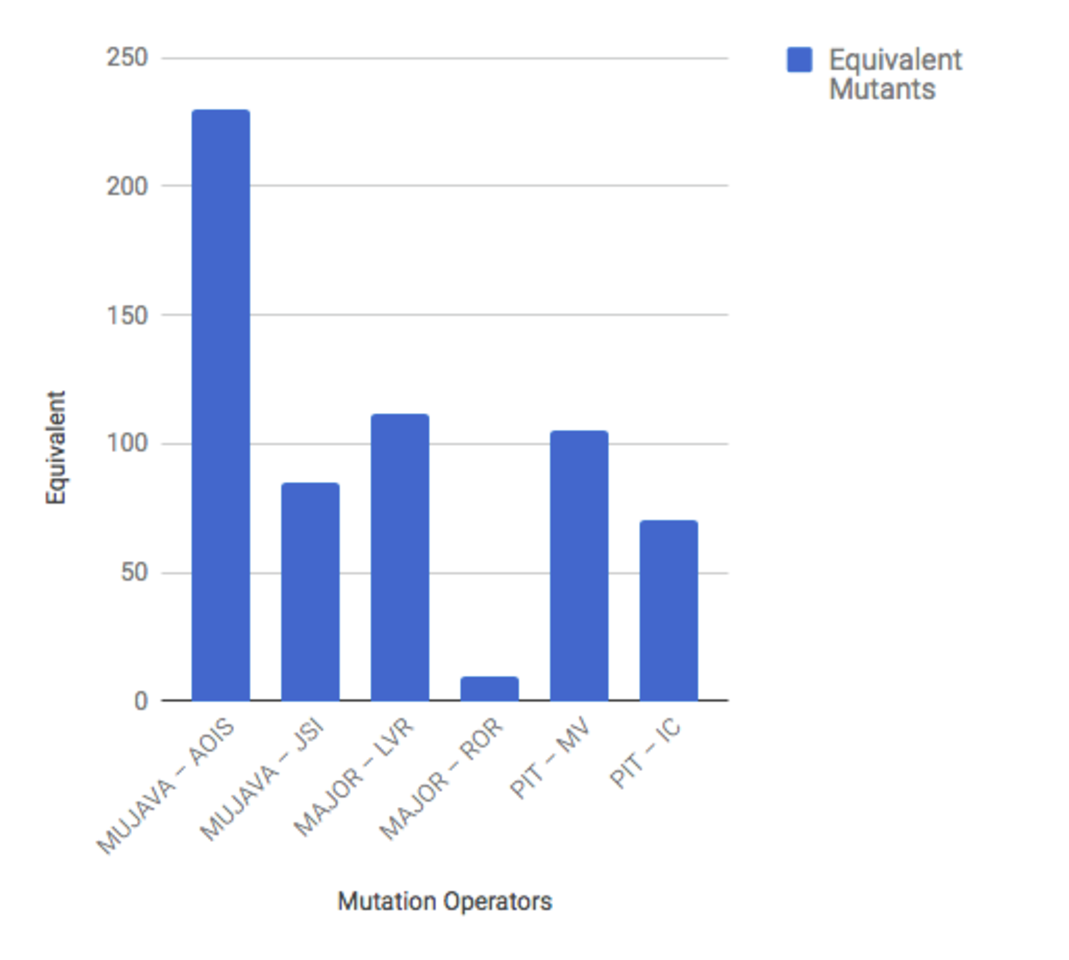
\includegraphics[scale=0.4]{images/EquivalentOperators.pdf}
% 			\label{fig:operators-equivalent}
% 		}
% 		\subfigure[Duplicated mutants based on some mutation operators.] {
% 			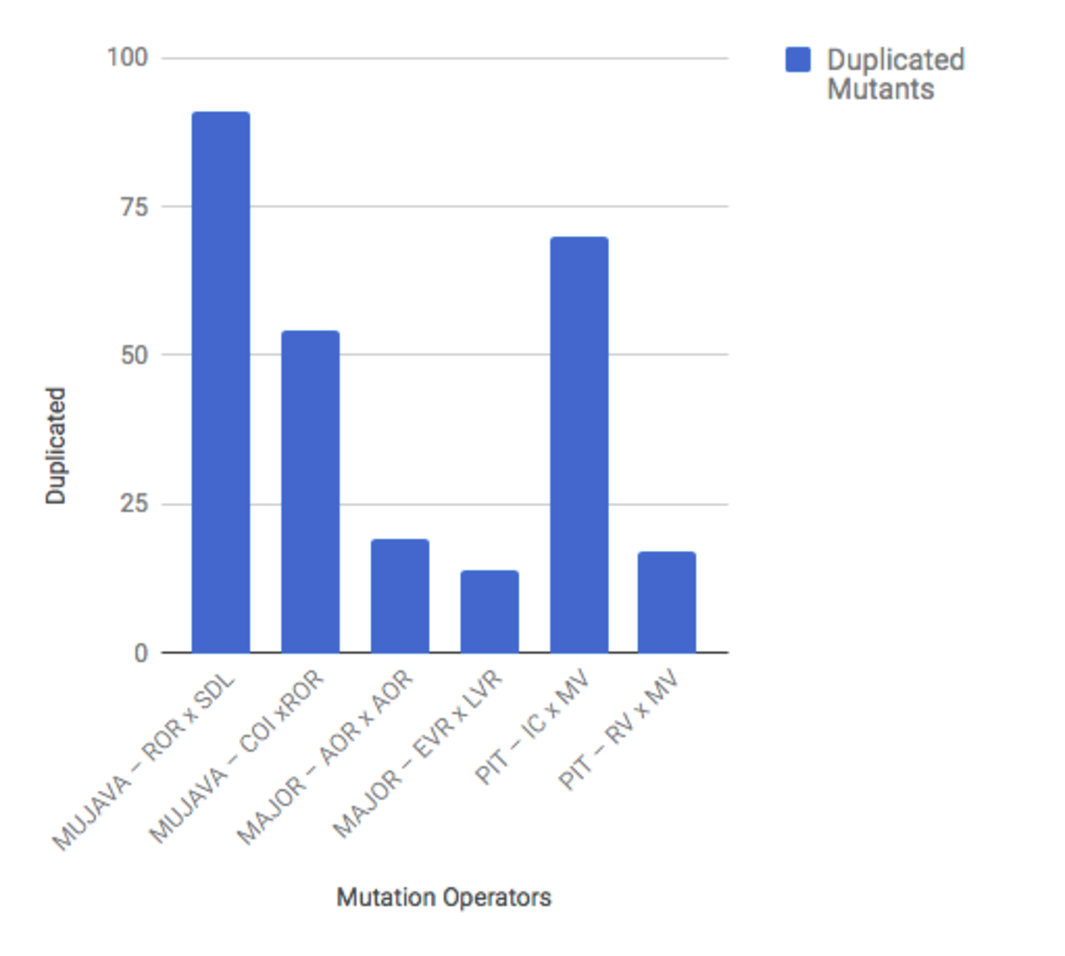
\includegraphics[scale=0.4]{images/DuplicatedOperators.pdf}
% 			\label{fig:operators-duplicated}
% 		}
		
% 		\caption{Equivalent and Duplicated mutants based on some mutation operators from the three mutation tools we used.}
		
% 	\end{center}
% \end{figure*}



This way, the answer to our research questions is yes, i.e., our strategy is capable of identifying useless mutants candidates. 
By using artificial and small Java programs, our strategy identified thousands of useless mutants with an accuracy of 95.92\% in our rating system.
%We do not know if our strategy would maintain the same performance using real programs, as we discuss in the Threats to Validity Section, but all this process is only the input to the real value of our work, that is deriving rules to avoid useless mutants.
Although the programs are simple, their mutants were crucial to derive those rules, as we shall see in Chapter~\ref{sec:rules}.


%\randoop{} did not generate a test to kill the mutants. For example, the JSI operator (Java Static Modifier Insertion) inserts the \texttt{static} keyword in class fields. In this case, \randoop{} could not generate a test to kill such mutants.

% \todo{
% For the mutants our strategy classified correctly as useless, but we could not derive rules, are the cases of coincidental correctness, that is, they are equivalent/duplicated, but at a very specific case we can not derive for a more general program.
% }

\subsection{Threats to Validity}
\label{sec:identifying-threats-to-validity}

The set of programs we used are based on a very few Java constructs. 
This is a threat to external validity. 
Still, this setup helped us to derive \NumberOfNewHeuristics new rules (Chapter~\ref{sec:rules}). 
In addition, the small programs allowed us to enable all available mutation operators from the three mutation tools we used in this work.

%Also, previous work could find bugs in refactoring engines (e.g., Eclipse, JRRT, and NetBeans) by using similar programs we used~\cite{SOARES:2010:1, SOARES:2013:1, MONGIOVI:2014:1, MELINA:2017:1}. 

Despite instantiating and executing the strategy only in Java programs, there is nothing particular to Java in our strategy. 
This means that it does not depend on the programming language. 
To use our strategy in other programming languages, all we need to do is to guarantee that everything is in the same language, i.e., programs, test suite, and mutants.

Our strategy identifies useless mutants candidates, which means it may lead to false positives. 
To weed out them, we rely on manual inspection, which is a threat. 
We minimized this threat by double checking all the useless candidates.

Another threat is that we set the \randoop{} time limit to three seconds. 
So, the tool has only three seconds to generate tests for a given program. 
In case we increase the time limit, we might reduce the number of false positives.

%\section{Introduction}
%\section{Better Discussion (RESULTS)}


\section{Research Status}
\label{sec:research-status-strategy}

We demonstrated that the strategy is capable of identifying useless mutants candidates.
However, we need to make some adjustments, add new features, and carry on the process improvement.

In what follows, we present the improvements we intend to perform.

\begin{enumerate}
    \item \textbf{Post-analysis: }We intend to add a \textit{post-analysis} in the final result of the strategy.
This post-analysis would try to extract information to facilitate the work of the programmer in deriving new rules.
For example, we could use a cluster algorithm to gather similar cases so as to indicate possible sites.
    \item \textbf{Execute the strategy with different instances: }We also intend to instantiate the strategy with different tools and setups.
For example, to derive more rules we intend to set our strategy to use different Java programs and different test suite generators (e.g., EvoSuite~\cite{FRASER:2011:1}).
    \item \textbf{Redundant Mutants: }Ammann et al.~\cite{AMMAN:2014:1} defines redundancy among mutants by identifying \textit{dominator mutants}, which subsume other mutants in the sense that mutant $m_i$ subsumes mutant $m_j$ if every test that kills $m_i$ also kills $m_j$. 
They demonstrated that a small set of mutants, approximately 1.2\%, subsumes all the others.
That is, approximately 99\% of all non-equivalent mutants are redundant.
%In \cite{PAPADAKIS:2016:1}, Papadakis et al. demonstrated that redundancy among mutants has a very good chance to inflate mutation score which puts in check all the studies that used such a metric.
\textit{Redundant mutants}, besides not adding anything to the mutation analysis, can inflate the mutation score \cite{PAPADAKIS:2016:1}, leading to misinterpretations about the outcome.
In summary, a small set of dominator mutants captures the power of the full set of mutants generated by a typical mutation system.
Redundant mutants could also be classified as useless.
As a next step we intend to adjust our strategy to classify redundant mutants candidates and extract rules to avoid them.
\end{enumerate}




%\subsection{Machine Learning}
%Machine learning allows a computer program to refine its decision-making abilities based on experience.

%Um outro passo que queremos discutir é a possibilidade de aliar técnicas de inteligência artificial a nossa estrategia, de maneira que a mesma possa aprender a derivar novas regras automaticamente, ou pelo menos dar fortes indicativos de descoberta de uma regra, a partir do que ela aprender olhando regras anteriores...







